\section{Ceph Components}

\begin{frame}{Ceph Cluster}
    \begin{figure}[htpb]
        \centering
        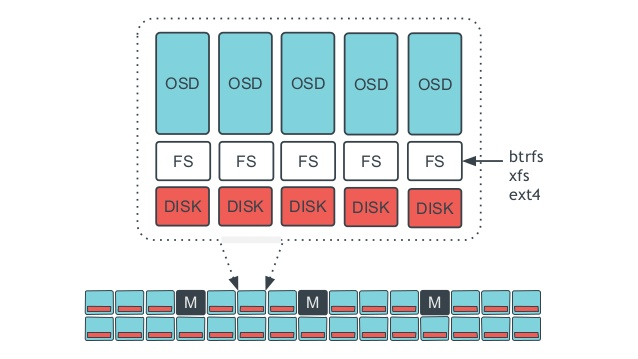
\includegraphics[width=0.8\linewidth]{cluster.jpg}
    \end{figure}
\end{frame}

\begin{frame}{Monitors}
    \begin{itemize}
        \item \textbf{Maintain the cluster map}
            \begin{itemize}
                \item MON map
                \item OSD map
                \item MDS map
                \item PG map
                \item CRUSH map
            \end{itemize}
        \item \textbf{Provide consensus for distributed decision making}
            \begin{itemize}
                \item Each MON knows about all the other MONs in the cluster
                \item First establish a quorum of more than half of MONs so an odd number of MONs is needed in the cluster
                \item MONs in a quorum can distribute maps to OSDs and clients. Clients request cluster maps from a MON only when the primary OSD fails
            \end{itemize}
        \item \textbf{Monitors are not in data path} 
    \end{itemize}
\end{frame}


\begin{frame}{Object Storage Node}
    \begin{itemize}
        \item \textbf{Object Storage Device (OSD)}
            \begin{itemize}   
                \item Building block of Ceph Storage Cluster
                \item One hard disk
                \item One Linux File System
                \item One Ceph OSD Daemon
            \end{itemize}
        \item \textbf{File System:}
            \begin{itemize}
                \item File system must be btrfs, xfs or ext4
                \item Have the XATTRs enabled
            \end{itemize}
   \end{itemize} 
\end{frame}

\begin{frame}{Ceph OSD Daemon}
    \begin{itemize}
        \item \textbf{Ceph Object Storage Device Daemon}
            \begin{itemize}
                \item Serve stored objects to clients
            \end{itemize}
        \item \textbf{OSD is primary for some objects}
            \begin{itemize}
                \item Responsible for replication
                \item Responsible for coherency
                \item Responsible for re-balancing
                \item Responsible for recovery
            \end{itemize}
        \item \textbf{OSD is secondary for some objects}
            \begin{itemize}
                \item Under the control of the primary
                \item Capable of becoming primary
            \end{itemize}
        \item \textbf{Supports extended objects classes}
            \begin{itemize}
                \item Atomic transactions
                \item Synchronization and notifications
                %\item Send computation to the data
            \end{itemize}
    \end{itemize}
\end{frame}

%\begin{frame}{xfs, btrfs, or ext4?}
%    
%\end{frame}

%\begin{frame}{Ceph Journal}
%   
%\end{frame}

\begin{frame}[t]{Ceph Stack}
    \begin{figure}[htpb]
        \centering
        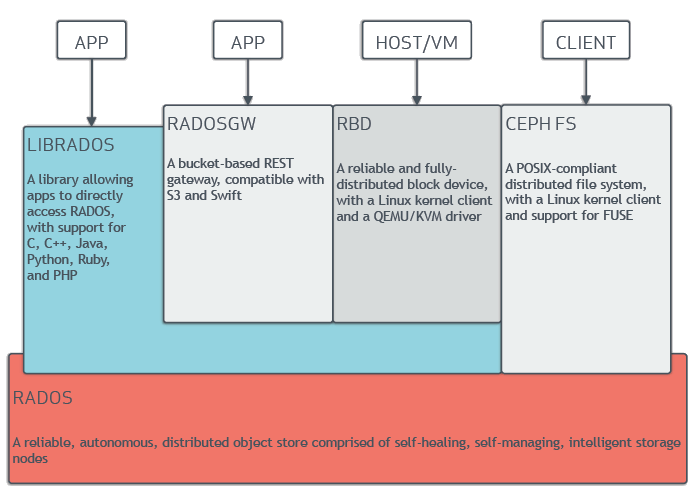
\includegraphics[width=0.75\linewidth]{stack.png}
        \caption{Ceph Stack}
        \label{fig:stack}
    \end{figure}
\end{frame}

\begin{frame}{Communication Methods}
    \begin{tabular}{|c|c|p{0.5\columnwidth}|}
    \hline
        \textbf{Ceph Service}    &   \textbf{Method}  &   \textbf{Description} \\
    \hline
        N/A &   \textit{librados}   &   Library that provides direct access to RADOS for applications \\
    \hline
        Ceph Object Gateway &   \textit{radosgw}    &   RESTful APIs for S3 and Swift compatibility \\
    \hline
        Ceph File System  &   \textit{libcephfs}  &   Library that provides access to Ceph Cluster via a POSIX-like interface \\
    \hline
        Ceph Block Device & \textit{librbd} &   Python module, provides file-like access to RBD images \\
    \hline
    \end{tabular}
\end{frame}

\begin{frame}{RADOSGW}
    \begin{figure}[htpb]
        \centering
        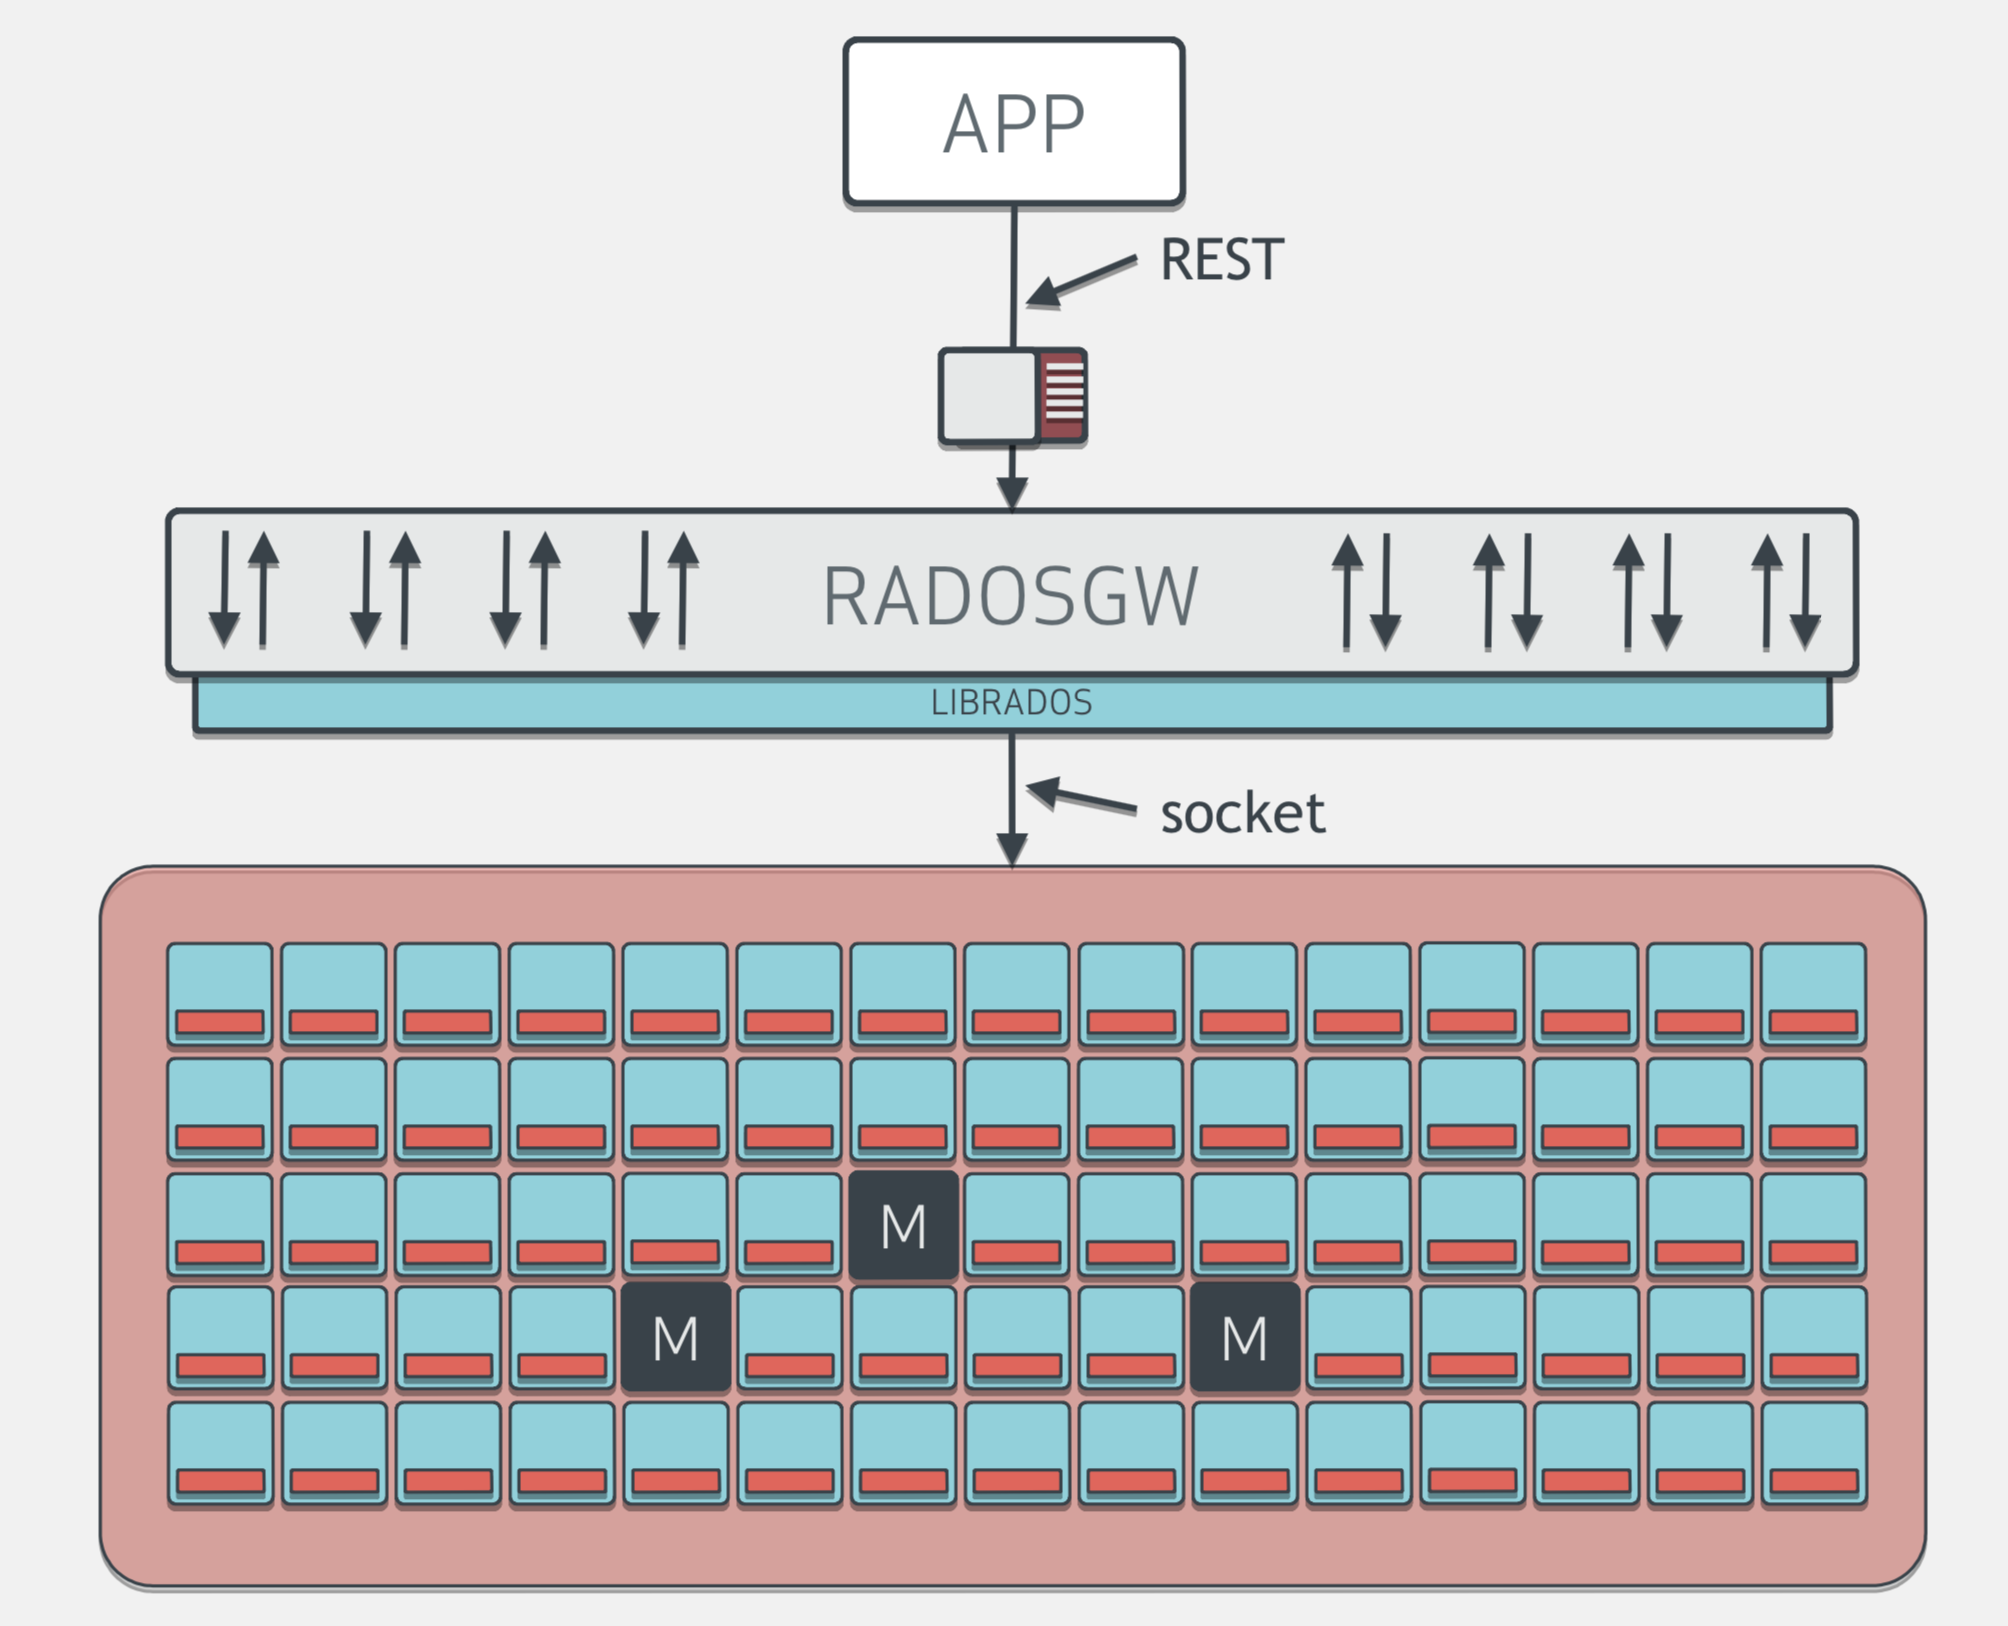
\includegraphics[width=0.7\linewidth]{rgw.png}
    \end{figure}
\end{frame}

\begin{frame}{RBD}
    \begin{figure}[htpb]
        \centering
        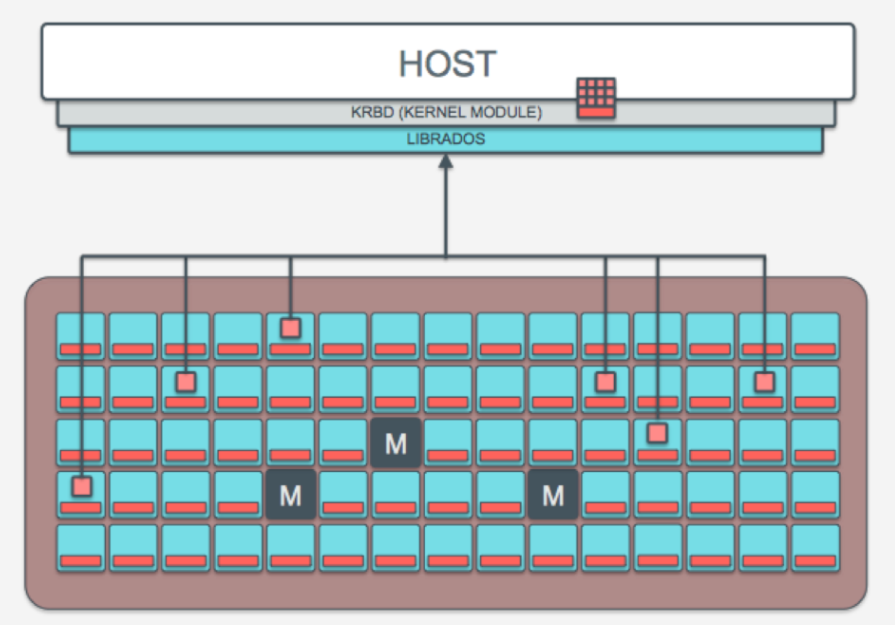
\includegraphics[width=0.8\linewidth]{rbd-native.png}
    \end{figure}
\end{frame}

\begin{frame}{Metadata Server(MDS)}
    \begin{itemize}
        \item \textbf{Manages metadata for a POSIX-compliant shared file system}
            \begin{itemize}
                \item Directory Hierarchy
                \item File Metadata(owner, timestamps, mode, etc)
                \item Stores metadata in Rados
                \item Does not access file content
                \item Only required for shared file system
            \end{itemize}
        \item \textbf{The Ceph Metadata Server daemon}
            \begin{itemize}
                \item Provides the POSIX information needed by file systems that enables CephFS to interact with the Ceph Object Store
                \item It remembers where data lives within a tree
                \item Client accessing CephFS data first make a request to an MDS, which provides what they need to get files from the right OSDs
            \end{itemize}
        \item If you aren't running CephFS, MDS daemons do not need to be deployed. 

    \end{itemize}
\end{frame}

\begin{frame}{CephFS}
    \begin{figure}[htpb]
        \centering
        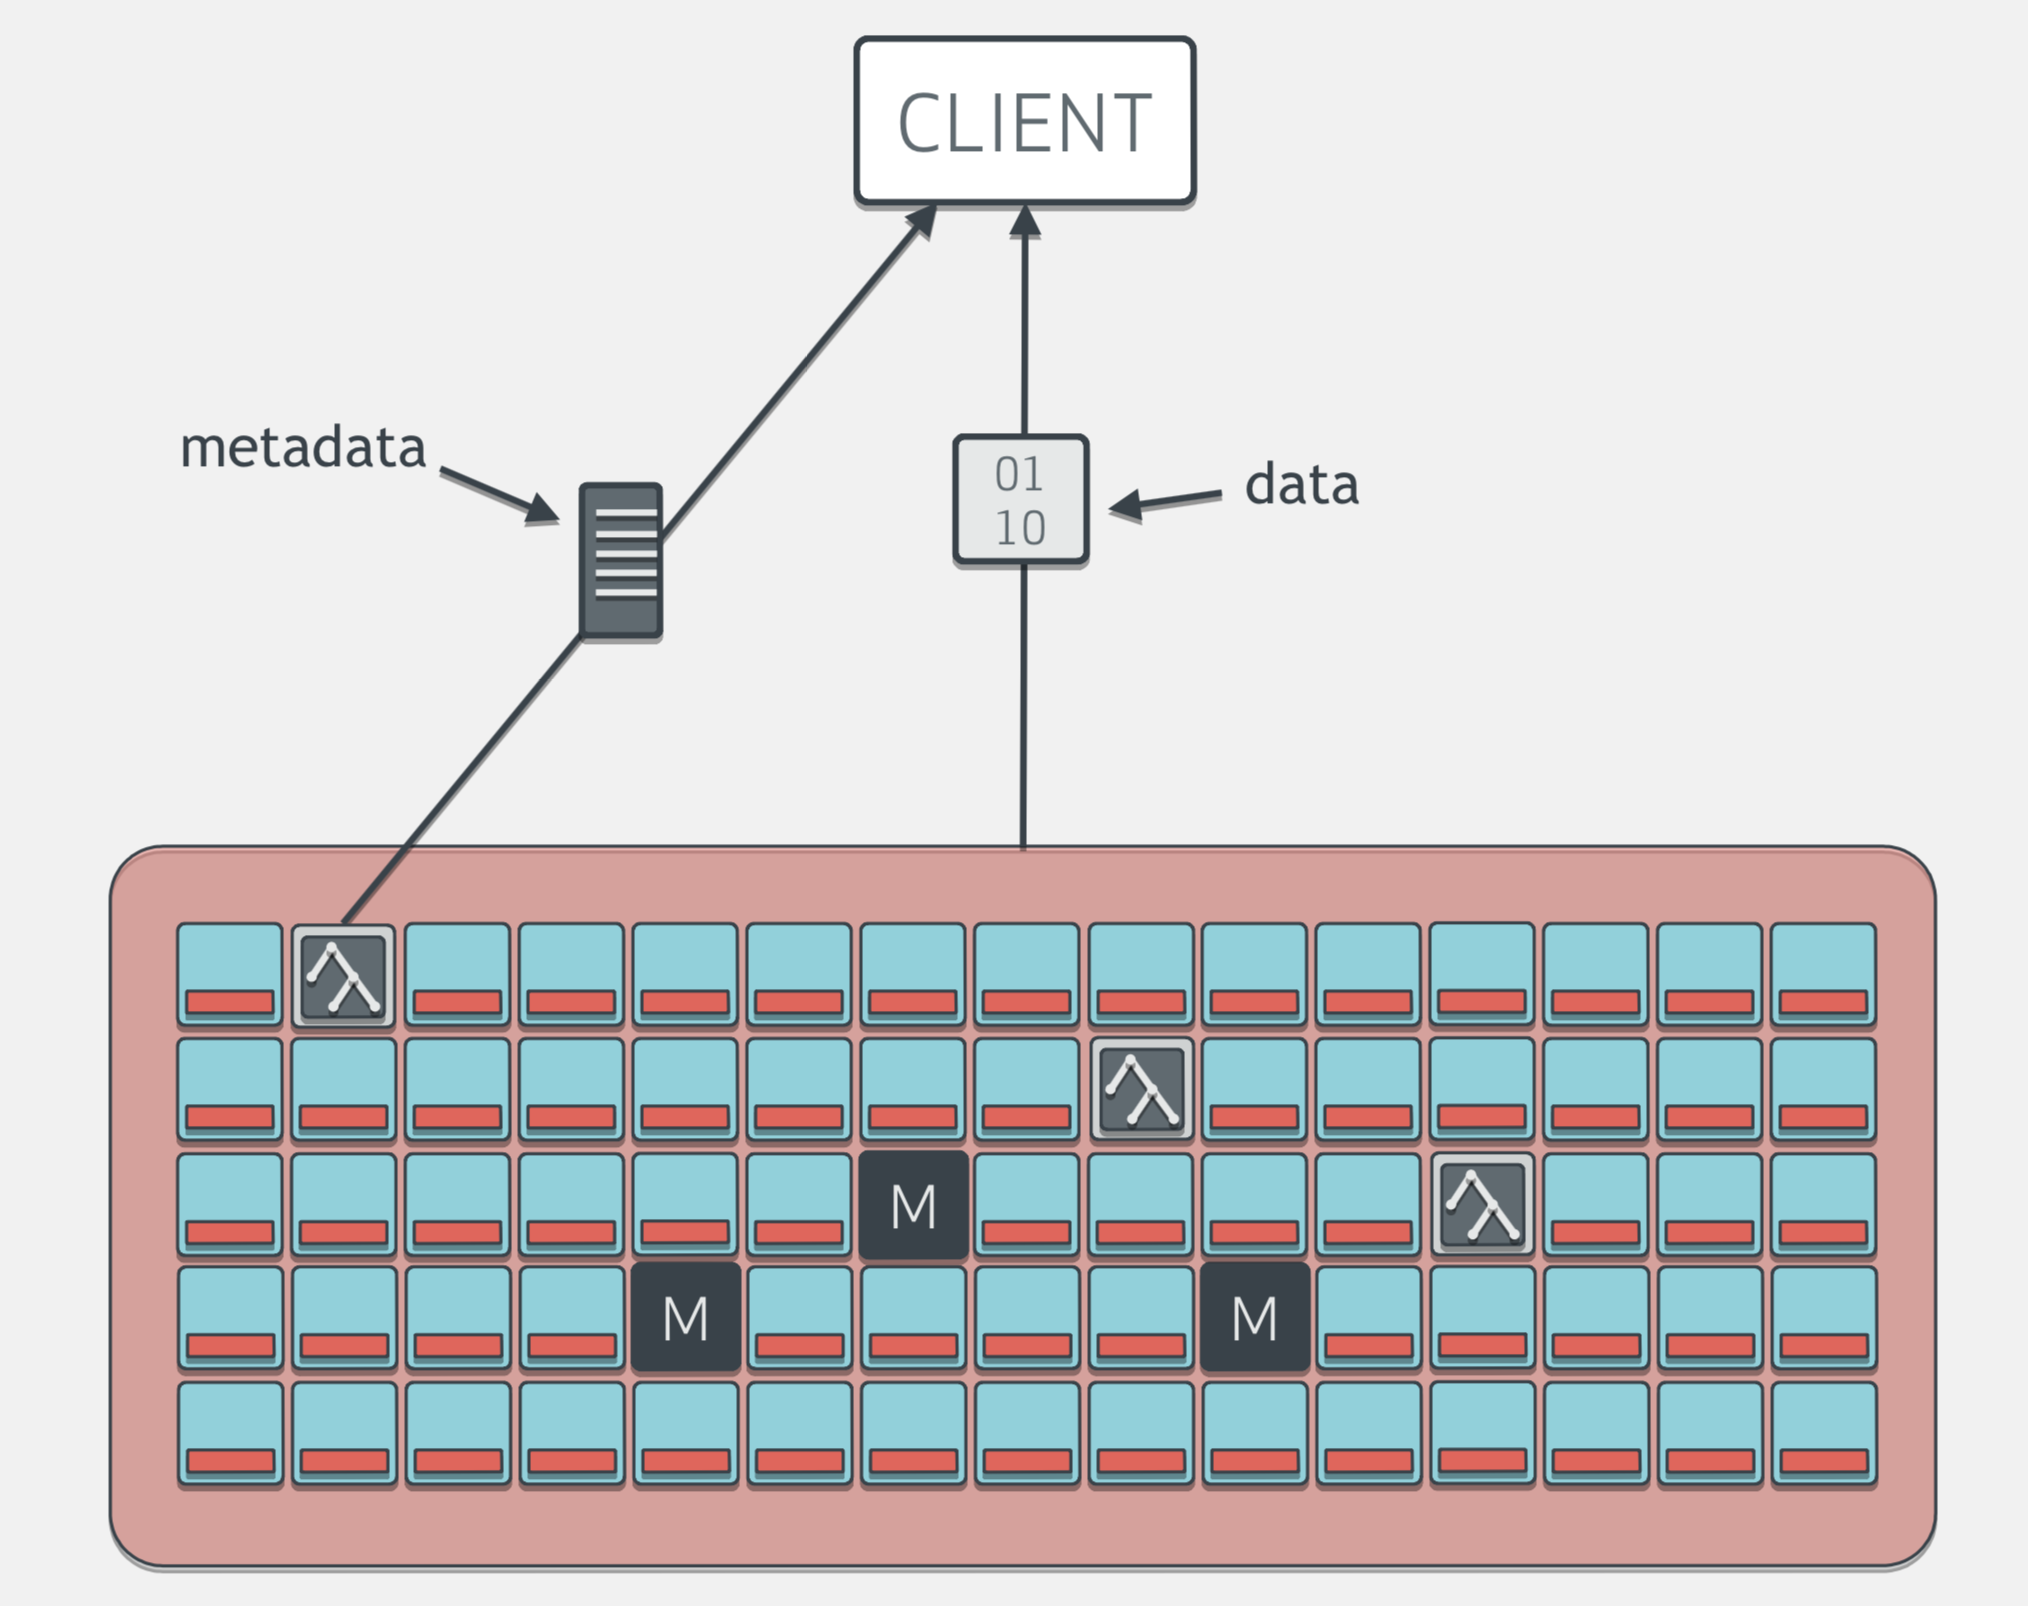
\includegraphics[width=0.7\linewidth]{cephfs.png}
    \end{figure}
\end{frame}

\begin{frame}[fragile]{Ceph Cluster}
\begin{lstlisting}[language=python]
ubuntu@ip-172-31-58-195:~# ceph -s
  cluster:
    id:     ccb00027-ca55-48cc-bf5a-b6cbf79c9b99
    health: HEALTH_OK

  services:
    mon: 3 daemons, quorum ip-172-31-56-105,ip-172-31-57-232,ip-172-31-58-195
    mgr: ip-172-31-56-105(active), standbys: ip-172-31-57-232, ip-172-31-58-195
    mds: cephfs-1/1/1 up  {0=ip-172-31-58-195=up:active}, 2 up:standby
    osd: 4 osds: 3 up, 3 in
    rgw: 1 daemon active

  data:
    pools:   8 pools, 184 pgs
    objects: 268  objects, 37 MiB
    usage:   3.1 GiB used, 87 GiB / 90 GiB avail
    pgs:     184 active+clean    
\end{lstlisting}
\end{frame}

\begin{frame}{Pools and Placement Groups}
    \begin{figure}[htpb]
        \centering
        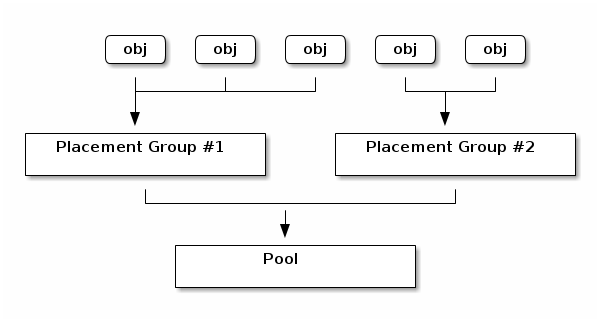
\includegraphics[width=0.8\linewidth]{placement-groups.png}
    \end{figure}
\end{frame}

\begin{frame}{Pools}
    \begin{itemize}
        \item \textbf{What are pools?}
            \begin{itemize}
                \item Pools are logical partitions for storing object data
            \end{itemize}
        \item \textbf{Pools have the following attributes:}
            \begin{itemize}
                \item Set ownership/access
                \item Set number of object replicas
                \item Set number of placement groups
                \item Set the CRUSH rule set to use
            \end{itemize}
        \item \textbf{The PGs within a pool are dynamically mapped to OSDs}
    \end{itemize}
\end{frame}

\begin{frame}[fragile]{Pools}
\begin{lstlisting}[language=python]
ubuntu@ip-172-31-58-195:~# ceph osd lspools
1 .rgw.root
2 default.rgw.control
3 default.rgw.meta
4 default.rgw.log
5 cephfs_data
6 cephfs_metadata
7 rbd
8 default.rgw.buckets.index
ubuntu@ip-172-31-58-195:~# rados df
POOL_NAME                    USED OBJECTS CLONES COPIES ... RD_OPS      RD WR_OPS     WR
cephfs_data                  28 B       2      0      6 ...      2   1 KiB      2  2 KiB
cephfs_metadata            13 KiB      22      0     66 ...      5   5 KiB     91 46 KiB
...
rbd                        37 MiB      19      0     57 ...   2522 5.3 MiB   1313 81 MiB

total_objects    268
total_used       3.1 GiB
total_avail      87 GiB
total_space      90 GiB 
ubuntu@ip-172-31-58-195:~#  ceph osd pool create {pool-name} {pg-num} [{pgp-num}]
\end{lstlisting}
\end{frame}

\begin{frame}{Placement Groups (PGs)}
    \begin{itemize}
        \item \textbf{What is a PG?}
            \begin{itemize}
                \item A PG is a logical collection of objects
                \item Objects within the PG are replicated by the same set of OSDs
            \end{itemize}
        \item \textbf{How to choose the PG?}
            \begin{itemize}
                \item An object's PG is determined by hashing the object name against the number of PGs in the pool
                \item A PG's location is determined by CRUSH according to desired protection and placement strategies
            \end{itemize}
    \end{itemize}
\end{frame}

\begin{frame}{Placement Groups (PGs)}
    \begin{figure}[htpb]
        \centering
        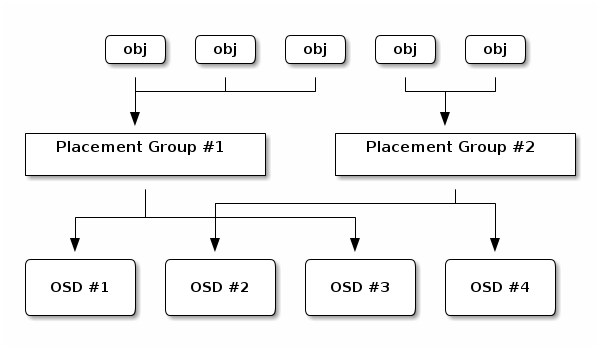
\includegraphics[width=0.8\linewidth]{pg2osd.png}
    \end{figure}
\end{frame}

\begin{frame}{Placement Groups (PGs)}
    \begin{itemize}
        \item \textbf{Without them}
            \begin{itemize}
                \item Track placement and metadata on per-object basis
                \item Not realistic nor scalable with a million++ objects
            \end{itemize}
        \item \textbf{Extra Benefits}
            \begin{itemize}
                \item Reduce the number of processes
                \item Reduce amount of per object metadata Ceph must track
            \end{itemize}
        \item \textbf{Handling the cluster life cycle}
            \begin{itemize}
                \item The total number of PGs must be adjusted when growing the cluster
                \item As devices leave or join the Ceph cluster, most PGs remain where they are
                \item Approximately 50-200 PGs per OSD is recommended -> to balance out memory and CPU requirements and per-OSD load
            \end{itemize}
    \end{itemize}
\end{frame}

\begin{frame}{From Object to OSD}
    \begin{figure}[htpb]
        \centering
        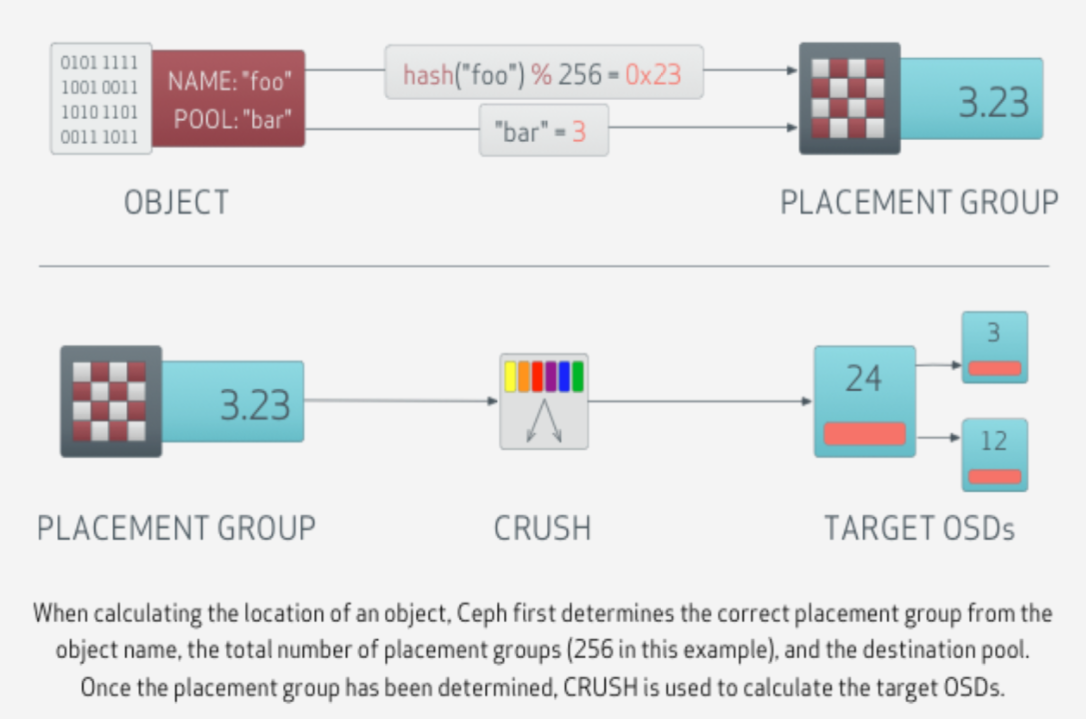
\includegraphics[width=0.8\linewidth]{object2osd.png}
    \end{figure}
\end{frame}
